Passing through the fog barrier, you stumble into a dream-like scene. The hallway ahead is identical to the one in which you were previously interred... but missing in sections, as if you were failing to picture the place in its entirety. You stand amongst a vast panorama of overcast sky and fog-choked environs: a flagstone island in the sky. A few emaciated corpses lay in soft repose around its wreckage.\\

A section of tile breaks loose, dropping to the mezzanine below with a loud crack.\\

The man from before emerges from the ruins as if summoned by the sound. At this distance, you can finally get a look as his face--and find it familiar. This man spoke the truth: he played some integral part in your life's story.\\

"Our champion has washed ashore. And now we shall assess the salvage."\\

The man turns his palms upwards, and a few of the corpses begin to stir.\\

\subsection*{Victory Condition}
Defeat Zealot Eóghainn

\subsection*{Doom Events}
\begin{itemize}
\item \textbf{Every 2nd Round:} \emph{Eóghainn steps into the fog.} Roll 2D6. Place Zealot Eóghainn on a hex located on either combination of the two dice scores. If neither location is valid, he remains in place.
\end{itemize}

\subsection*{Encounter Table}
\begin{tcolorbox}
\textbf{Roll:} 1D6
\begin{center}
\begin{tabular}{ L | L | L }
\multicolumn{1}{c|}{\textbf{1}} & 
\multicolumn{1}{c|}{\textbf{2}} & 
\multicolumn{1}{c}{\textbf{3}} \\
\emph{Secret Parable} &
\textbf{A:} \emph{Secret Word}\newline \textbf{B:} \emph{Open-Palm Slap}\newline \textbf{C:} \emph{Secret Chant} &
\textbf{A:} \emph{Open-Palm Slap}\newline \textbf{B:} \emph{Secret Word} \\
\hline
\multicolumn{1}{c|}{\textbf{4}} & 
\multicolumn{1}{c|}{\textbf{5}} & 
\multicolumn{1}{c}{\textbf{6}} \\
\textbf{A:} \emph{Open-Palm Slap}\newline \textbf{B:} \emph{Secret Word} &
\textbf{A:} \emph{Secret Word}\newline \textbf{B:} \emph{Open-Palm Slap}\newline \textbf{C:} \emph{Secret Chant} &
\emph{Secret Parable} \\
\end{tabular}
\end{center}
\textbf{Note:} Each round, all Risen Prisoner enemies will Move towards the character and attempt \emph{Swipe}.
\end{tcolorbox}

\subsection*{Enemy Sheets}
\hrule
\ \\
{\large \textbf{Zealot Eóghainn}}\\\\
\begin{tabular}{s s s}
\textbf{HP:} 8 & \textbf{Move:} 2\\
\textbf{L.DEF}: 3 & \textbf{D.DEF:} 2\\
\end{tabular}\\

\emph{Intelligent:} This entity is human, or possesses a human-like intellect.\\

\textbf{Attacks:}
\begin{itemize}
\item \emph{Open-Palm Slap} -  Inflict Stun on an adjacent entity.
\item \emph{Secret Word} - Deal 1 \emph{Inevitable} Smite damage to an entity within 2-4 tiles.
\item \emph{Secret Chant} - Add 1 Enhanced Defense: \textbf{P.DEF} (1) condition token to this enemy sheet.
\item \emph{Secret Parable} - Roll 2D6. Place a Risen Prisoner on a hex located on either combination of the two dice scores. If neither location is valid, there is no effect.
\end{itemize}
\hrule
\ \\
{\large \textbf{Risen Everloyal}}\\\\
\begin{tabular}{s s s}
\textbf{HP:} 3 & \textbf{Move:} 4\\
\end{tabular}\\

\emph{Undead:} This entity ignores Bleed and Dark damage, and the Bleeding, Charmed, Maddened, and Fear conditions.\\

\textbf{Attack:}
\begin{itemize}
\item \emph{Swipe} - Deal 1 \emph{Unparryable} Crush damage to an adjacent entity.
\end{itemize}

\pagebreak

\subsection*{Encounter Map}
\begin{center}
\framebox{
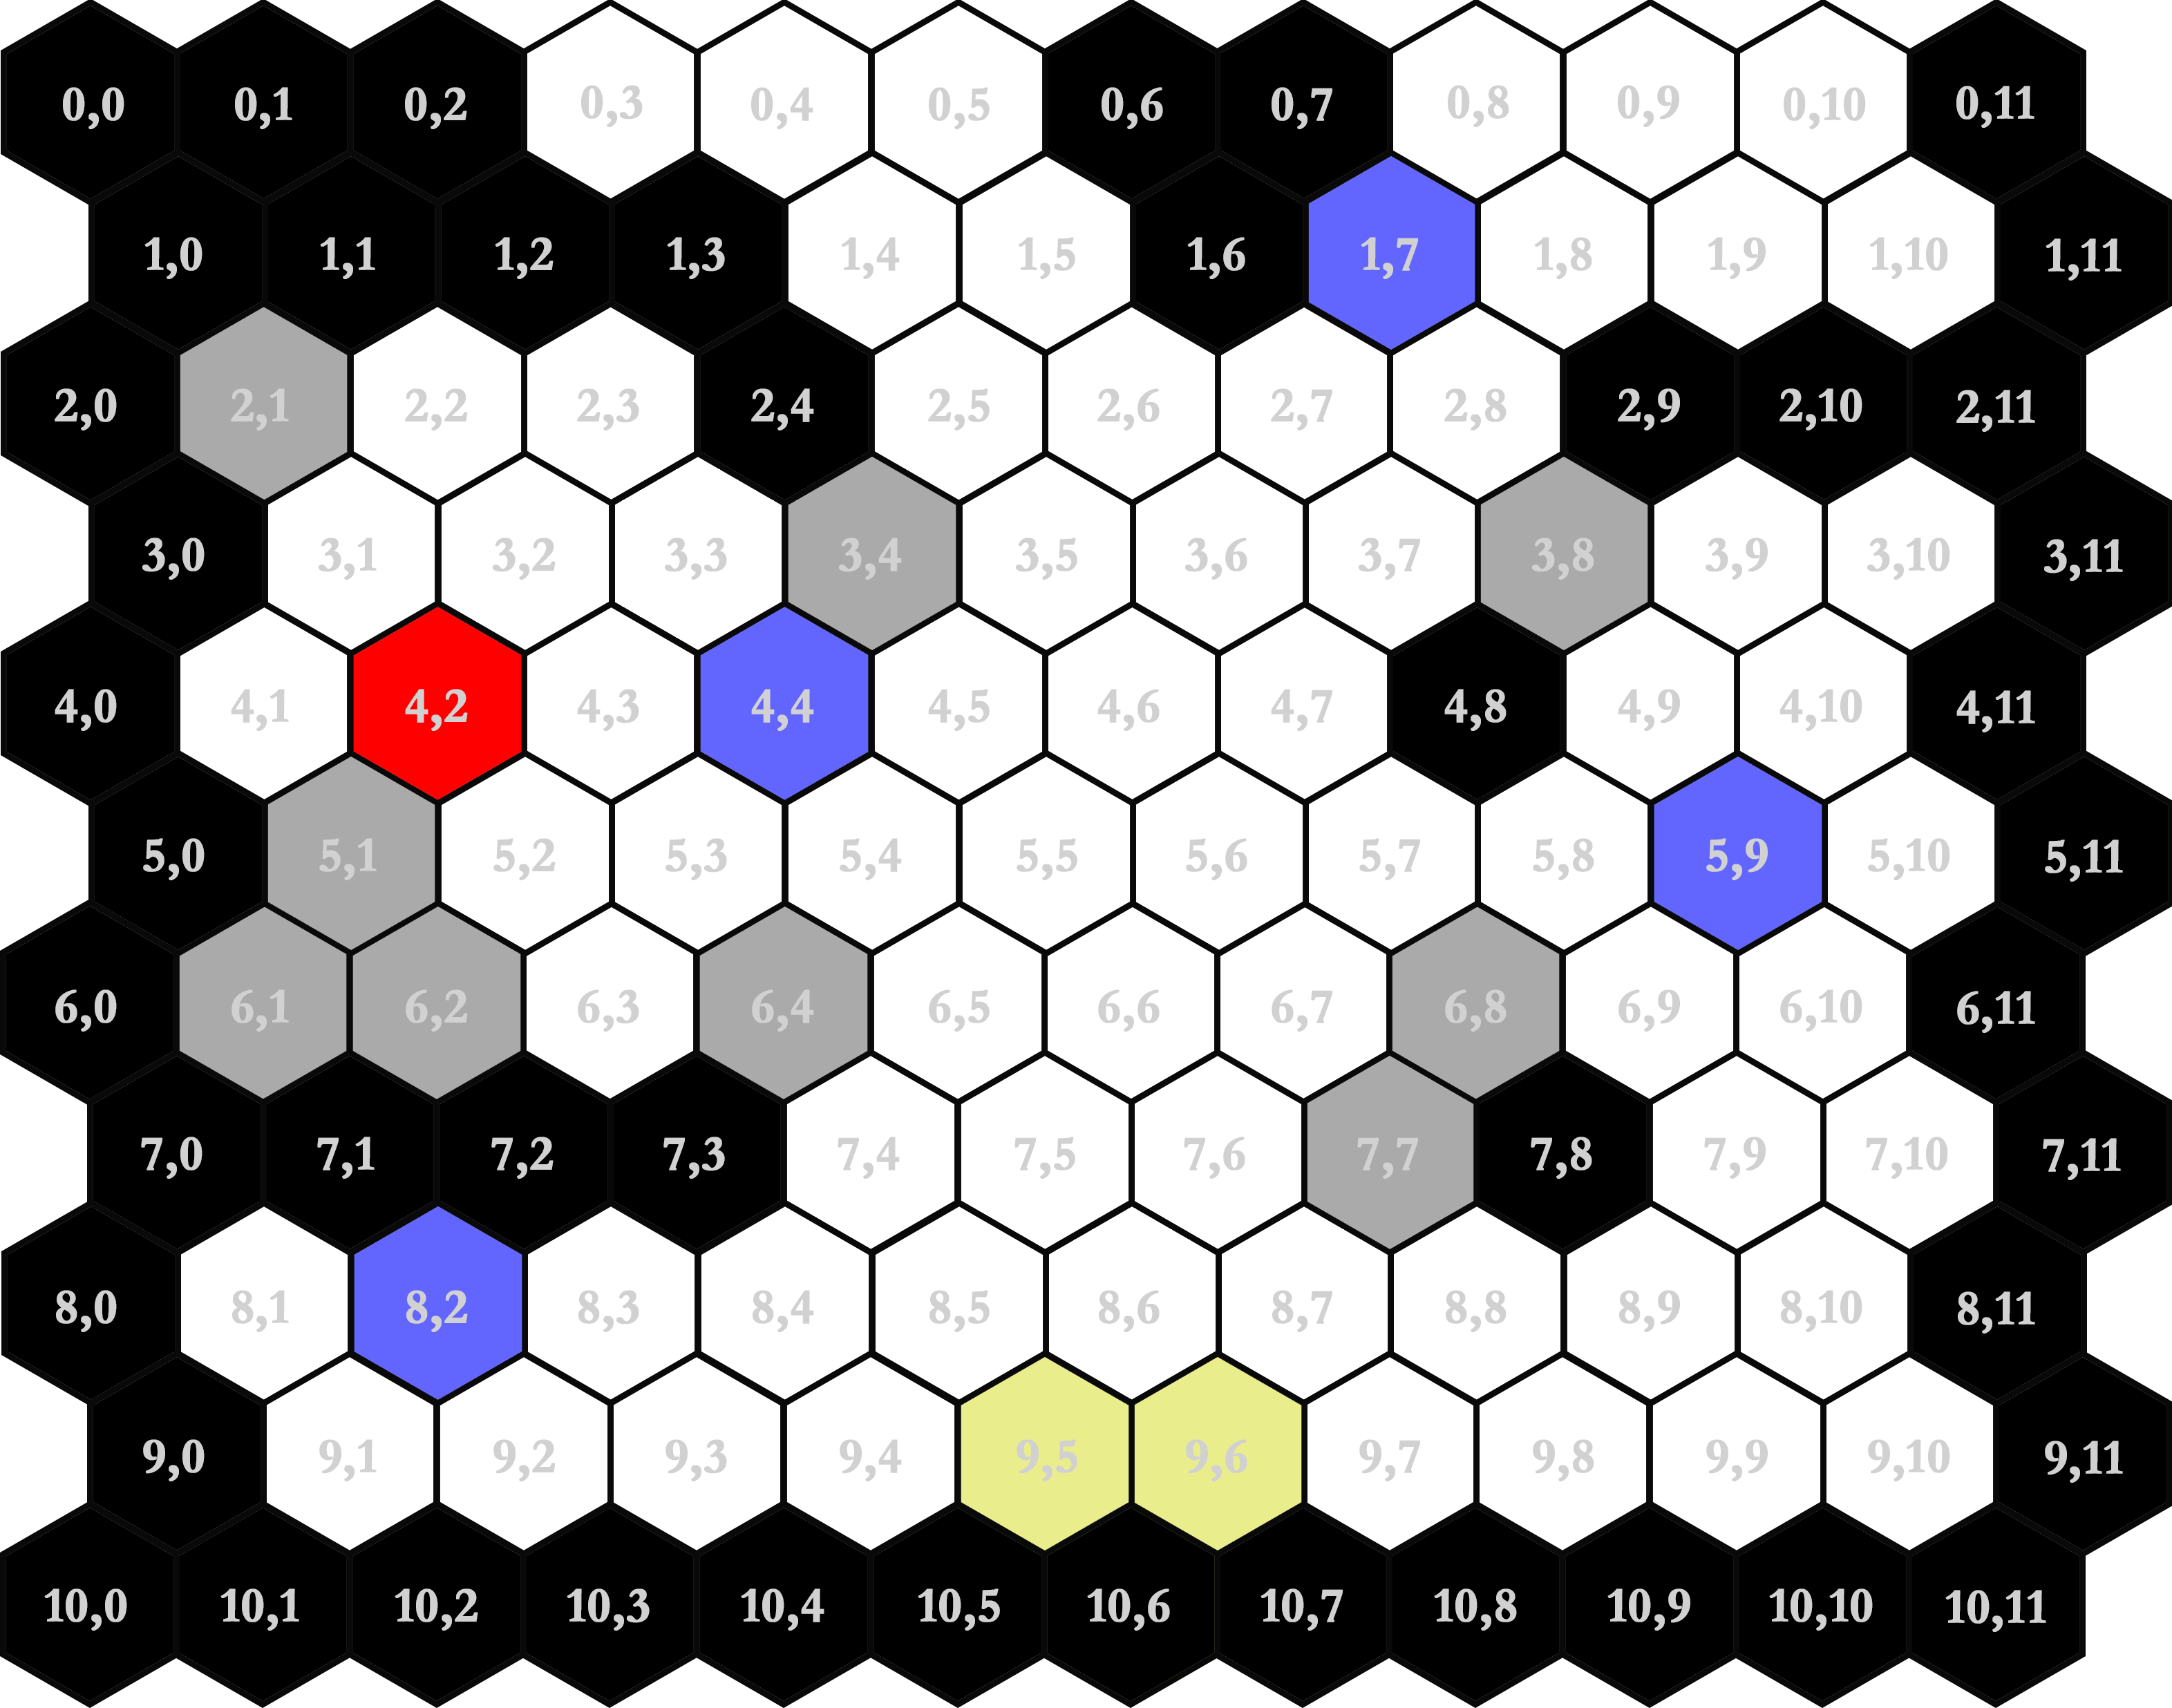
\includegraphics[width = 0.96\textwidth]{./maps/c317.png}
}
\end{center}

\subsection*{Setup Instructions}
\begin{itemize}
\item \textbf{Goldenrod:} Character Start Location. Place the character on either tile.
\item \textbf{Red:} Enemy Start Location. Place Zealot Eóghainn on this tile.
\item \textbf{Blue:} Enemy Start Location. Place a Risen Prisoner on \emph{two} of these tiles.
\item \textbf{Black:} Impassable Boundary/Full-Cover
\item \textbf{Light Gray:} Half-Cover.
\end{itemize}

\pagebreak

\subsection*{Victory}
The man stumbles backwards a few steps, then drops to a knee and clutches his side.\\

“Very well.”\\

He gasps and pants.\\
“Ye have... \emph{haa}... rightfully reassumed the mold that begotten ye. \emph{Haa}... \emph{haa}...”\\

He rakes a forearm across his brow, plastering its arm hairs against his skin, then stands.\\

\notegain{c317a} Zealot Eóghainn has assessed His champion\\
>> \turnto{c317x1}

\subsection*{Defeat}
You lay in defeat. A trio of risen corpses shamble towards you with grasping hands. Then the man raises his arms, and they collapse in place.\\

“A valiant attempt. But just an attempt, nonetheless.”\\

The man approaches you with a hand outstretched, and lifts you onto your feet.\\

\notegain{c317b} Zealot Eóghainn has assessed His champion\\
>> \turnto{c317x1}